%!TEX TS-program = xelatex
%!TEX encoding = UTF-8 Unicode
\documentclass[handout]{beamer}
\usetheme{CambridgeUS} % replace it with Boadilla if you want no section bar
%\usecolortheme{crane} % other ones: dove, dolphin, rose, seahorse, orchid, crane, seagull, lily, wolverine
%\usefonttheme{serif} 
\usefonttheme[onlymath]{serif} % uncomment if you want it just for math

\setbeamertemplate{navigation symbols}{}  % comment to have nagivation

\usepackage[compress,comma,authoryear]{natbib}
\usepackage{tikz}
\usetikzlibrary{mindmap,trees}
\usepackage{amsmath,mathtools}
\usepackage{amsthm}
\usepackage{booktabs}
\usepackage{graphicx,epstopdf}
\usepackage{hyperref}
\usepackage{fontspec}
\newfontfamily{\FA}{XB Niloofar}[Extension = .ttf] % Farsi
\newfontfamily{\FAN}{IranNastaliq}[Extension = .ttf] % Farsi Nastaliq

\definecolor{blue}{RGB}{0,114,178}
\definecolor{red}{RGB}{213,94,0}
\definecolor{yellow}{RGB}{240,228,66}
\definecolor{green}{RGB}{0,158,115}
\definecolor{Lblue}{RGB}{0,197,155}
\definecolor{Dblue}{RGB}{0,76,119}
\definecolor{Lgreen}{RGB}{180,255,230}

\hypersetup{
	colorlinks=false,
	linkbordercolor = {white},
	linkcolor = {blue}
}
\definecolor{MyBackground}{RGB}{245,245,245}

\setbeamercolor{frametitle}{fg=blue}
\setbeamercolor{title}{fg=blue}
\setbeamertemplate{footline}[frame number]
\setbeamertemplate{navigation symbols}{} 
\setbeamertemplate{itemize item}[circle]%{$\bigstar$}
\setbeamertemplate{itemize subitem}{$\bigstar$}
\setbeamercolor{itemize item}{fg=blue}
\setbeamercolor{itemize subitem}{fg=blue}
\setbeamercolor{enumerate item}{fg=blue}
\setbeamercolor{enumerate subitem}{fg=blue}
\setbeamercolor{button}{bg=MyBackground,fg=blue}
\setbeamercolor*{palette primary}{use=structure,fg=blue,bg=white}
\setbeamercolor*{palette secondary}{use=structure,fg=white,bg=Dblue}
\setbeamercolor*{palette tertiary}{use=structure,fg=white,bg=blue}
\setbeamercolor*{palette quaternary}{fg=white,bg=black}
\setbeamercolor*{palettes quaternary}{fg=white,bg=Lgreen}
%\setbeamercolor{titlelike}{parent=structure,bg=Lgreen}
%\setbeamercolor{title in head/foot}{bg=Lgreen,fg=orange}

\setbeamertemplate{enumerate item}{%
	\usebeamercolor[bg]{item projected}%
	\raisebox{1.5pt}{\colorbox{blue}{\color{fg}\footnotesize\insertenumlabel}}%
}



\usetikzlibrary{fit,positioning}

\newenvironment{transitionframe}{
	\setbeamercolor{background canvas}{bg=MyBackground}
	\begin{frame}}{
	\end{frame}
}

\begin{document}
	\title[Econometrics 2]{Econometrics 2 (M.Sc.)}
		\subtitle{Causality}
		\author[Mohammad Hoseini]{Mohammad Hoseini}
		
	\date[Spring 2024]{Spring 2024 \\
	\vspace{10pt} @metrics2
}

\begin{frame}[plain]
	\titlepage
\end{frame}

\begin{transitionframe}[plain,noframenumbering]

		 \color{blue} 
		\qquad \qquad \qquad $\underset{\downarrow}{\text{research question}}$
	\begin{center}		
		\huge
		{\FA
		پی؟ \ \ فرخنده \ \ ای \ \ می‌آیی \ \ کجا \ \ از \qquad  هی \ \ که \ \ را \ \ اشتر \ \ پرسید \ \ یکی \ \ آن
		
		تو \ زانوی \ از \ پیداست \ خود \ گفت  \qquad تو \ کوی \ گرم \ حمام \ از \ گفت 
		}
	\end{center}
	
	 \hspace*{3cm} $\overset{\uparrow}{\text{empirics}}$\hspace*{3.5cm}  $\overset{\uparrow}{\text{theory}}$
\end{transitionframe}

\section{Causality }
\subsection{Introduction}

\begin{frame}{Introduction}
What is causal relationship?\bigskip\pause

``The falling out of trees sleeves is the cause of going to school''. Is this statement reasonable?\pause\bigskip

Without theory no causal relationship is defined.\bigskip

How much $y$ is caused by $x_1$ and how much by $x_2$?\bigskip


\end{frame}

\begin{frame}{Correlation does not mean causation}
	\begin{center}
		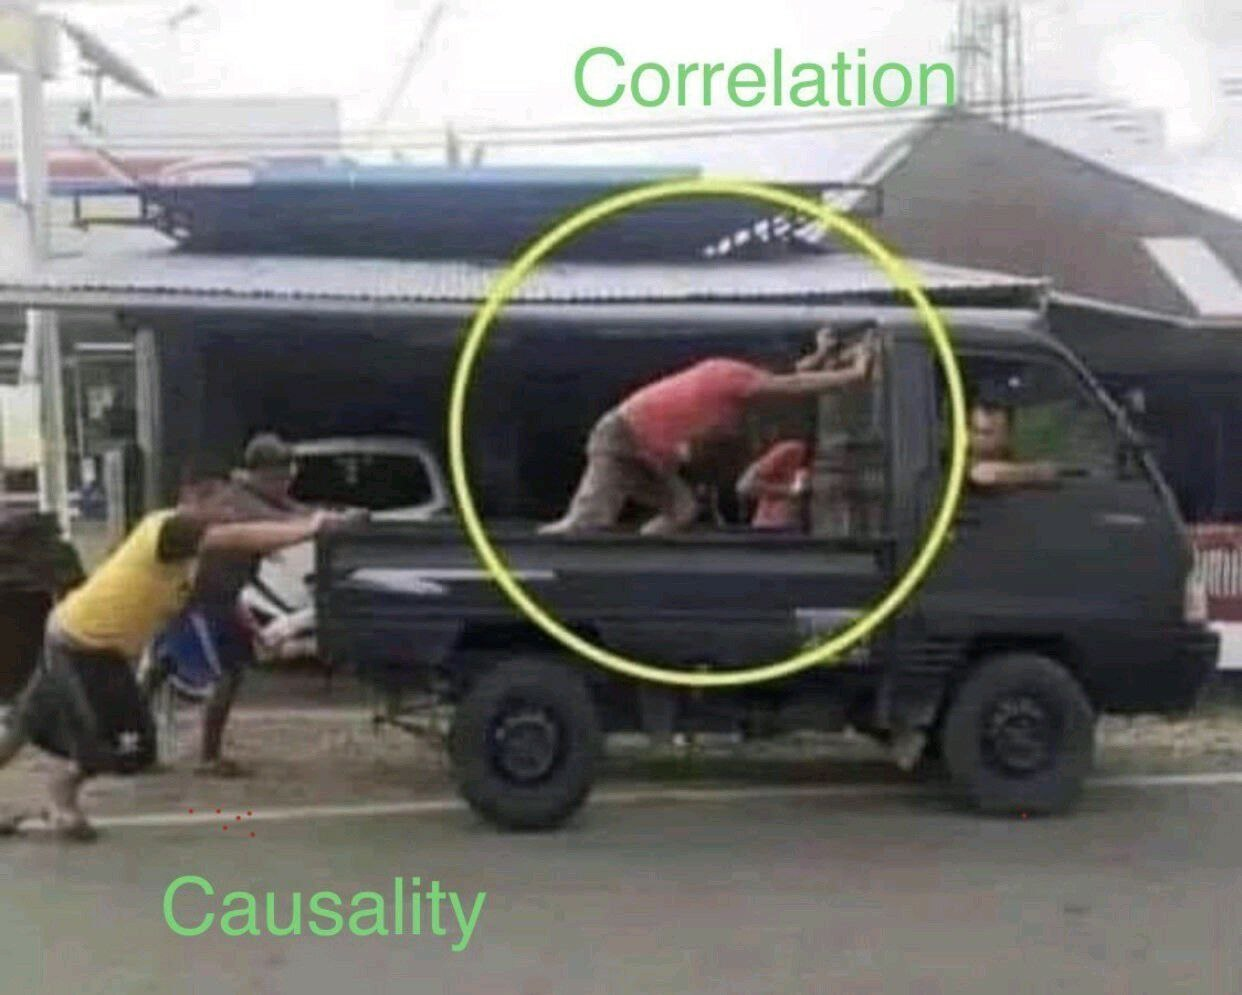
\includegraphics[width=.75\linewidth]{./Figures/corrvscause.jpg}
	\end{center}
\end{frame}

\begin{frame}{Causality in econometrics}
Different paradigms for causality in econometrics
\begin{itemize}
	\item Probabilistic: Structural estimation (Cowell commission), Granger causality, SVAR, Graph theory models, etc.
	\item Counterfactualist: Potential Outcome Model (Rubin Causal Model)
\end{itemize}\bigskip

%\textbf{Potential Outcome Model} is the focus of this course.

A model consists of 
\begin{enumerate}
	\item A set of variables $W$ with a joint probability distribution $F(W)$.
	\item A theory to order variables into cause and effect
	\item Functional forms for specifying the parameters of the model.
\end{enumerate}\bigskip
The most controversial step is the theory: assuming an a priori ordering of variables into causes (exogenous variables) and effects (endogenous variables).
\end{frame}

\begin{frame}{Causality in structural models}
Exogeneity: $f(W|\theta)=f_1(Y|Z,\theta_1)f_2(Z|\theta_2)$\medskip

Knowledge of $f_2(Z|\theta_2)$ is not required for inference on $\theta_1$ and we can validly condition the distribution of Y on Z.\bigskip

We usually justify the exogeneity assumption by a theory. Sometime we accept this, sometime we test it.\medskip

Common exogenous variables: natural experiments, government interventions, innate characteristics etc.

\end{frame}


\begin{frame}{Impact assessment and program evaluation}
We have especial interest on causal inference on the impact of policies or private decisions on an outcome variable
\begin{itemize}
	\item Transfer payment on labor supply
	\item Years of schooling on wage
	\item Class size on student learnings
	\item Health insurance on utilization of health care
	\item \dots

\end{itemize}\bigskip

Using only observational data poses many challenges to address these questions.
\end{frame}

\begin{frame}{Potential outcome models}
Since the early 1990, the potential outcome approach has gradually become the dominant framework for analyzing causality.\medskip

How can we estimate a causal relationship between $D$ and $y$?
%\pause
%
%\begin{enumerate}
%	\item How much $y$ changes if $D$ is changed randomly so that observation with different $D$ are otherwise comparable, or \pause
%	\item How much $y$ changes if $D$ is changed in a perfectly-controlled environment
%\end{enumerate} \pause
%\bigskip
Example: \begin{itemize}
	\item $D$ going to school (binary) or years of schooling (continuous)
	\item $y$ income as adult
\end{itemize}

\end{frame}


\subsection{Overview of the methods}


\begin{frame}{Example: vocational training}
A 6 week vocational training program to help unemployed individuals to find a job.\medskip

What is the effect of the program?\medskip

\begin{itemize}
	\item $y_i$ denote employment status of individual $i$
	\item $D_i=1$ if $i$ attended the program and $D_i=0$ otherwise
	\item $T$ is set of people who attended, and $C$ is those who did not
\end{itemize}\medskip

We have survey data on workers after the introduction of program.  \medskip\pause

Compare the proportion of employed among attendants and those who did not: \[\frac{1}{N_T}\sum_{i\in T}y_i>? \frac{1}{N_C}\sum_{i\in C}y_i\]


\end{frame}


\begin{frame}{Example cont'd}

Consider the regression \begin{equation}\label{e1}
y_i=\alpha+\beta D_i+e_i
\end{equation}

For the moment, assume $E[e_i|D_i=1]=E[e_i|D_i=0]=E[e_i]=0$: \begin{itemize}
\item $E[y_i|D_i=0]=\alpha$
\item $E[y_i|D_i=1]=\alpha+\beta$
\item[$\Rightarrow$] treatment effect:  $E[y_i|D_i=1]-E[y_i|D_i=0]=\beta$
\end{itemize}\medskip

Comparing the proportion of employed among attendants and those who did not is equivalent to estimating $\beta$: \[\frac{1}{N_T}\sum_{i\in T}y_i>? \frac{1}{N_C}\sum_{i\in C}y_i \ \Leftrightarrow \ \beta>? \ 0 \]

\end{frame}

\begin{frame}{Example cont'd}


We find more unemployment among those who attended the program: \begin{itemize}
\item $\frac{1}{N_T}\sum_{i\in T}y_i< \frac{1}{N_C}\sum_{i\in C}y_i \ $   or   $\ \beta< 0$ 
\end{itemize}\medskip

What is going on?\medskip

\pause

Women and young workers normally have a higher unemployment rates.\medskip

It is reasonable to assume they are overrepresented in the training.  \medskip
\pause

Control for gender and age. $x_i$ is vector of worker characteristics:
\begin{equation}\label{e2}
y_i=\alpha+\beta D_i+\gamma x_i+ e_i
\end{equation}
Again we find $\beta<0$. What is going on?
\end{frame}



\begin{frame}{Example cont'd}
Workers who have difficulty finding (keeping) a job are more likely to be unemployed, and attend the program.
\medskip

But we don't observe the ability of individuals to find or keep a job.  
What can we do?
\pause\medskip

Suppose we observe workers over time; before and after the introduction of the program ($t=1,2$).\medskip


We can estimate a regression with individual dummy $\alpha_i$ and time dummy $\delta_t$
\begin{equation}\label{e3}
y_{it}=\alpha_i+\beta D_{it} +\gamma x_{it} +\delta_t+e_{it} \end{equation}

We now obtain $\beta>0$.  Say it is 5\%.
\end{frame}

\begin{frame}{Example cont'd}
Can we say the effect of the training program is a 5\% increase in the probability of finding a job?
\pause
\medskip

Not really!  
Individuals who know they benefit more from the program are more likely to enroll.\medskip


Hence $\beta$ is probably an overestimate of the benefit for a random worker.
\pause\medskip

To solve this problem we can randomise the program:  Some individuals are randomly selected and given the training, while others are not.  \medskip

We observe these individuals before and after the program, and estimate\begin{equation}\label{e4}
y_{it}=\alpha_i+\beta D_{it} +u_{it}
\end{equation}
We obtain $\beta=0.5\%$.
\end{frame}

\begin{frame}{Example cont'd}
$\beta=0.5\%$ is the benefit for a randomly selected worker (ATE).\bigskip

Why this number is low?\medskip\pause

Because it mixed individuals who benefit little with those who benefit a lot.\bigskip

To investigate this further, we can estimate:
\begin{equation}\label{e5}
y_{it}=\alpha_i+\beta D_{it} +u_{it}
\end{equation}
For young workers only. We get $\beta=3\%$.\medskip

Similarly, $\beta=6\%$ for young women.
\end{frame}

\begin{frame}{Vocabulary}
We want to know the treatment effect
\begin{itemize}
\item Regression (\ref{e1}) is a simple difference in means (diff)
\item Regression (\ref{e2}) controls for selection on observables
\item Regression (\ref{e3}) is a diff-in-diff and controls for unobservables
\item Regression (\ref{e4}) is a randomized field experiments
\item Regression (\ref{e5}) uses only a subset of the target population and estimates heterogeneous effects (treatment effects that differ across individuals)	
\end{itemize}\medskip

The difficulty of causal inference is the absence of counterfactual\medskip


We wish to know what would have happened if someone who did not receive the treatment, had in effect received it.
\end{frame}


\begin{frame}{Formalizing the potential outcome model}

Assume $y_i$ is the outcome for individual $i$
\begin{itemize}
	\item $y_i^0$: outcome if $i$ is NOT under treatment
	\item $y_i^1$: outcome if $i$ is under treatment
	\item $D_i$: whether the individual is treated ($D_i=1$) or not ($D_i=0$)
\end{itemize}\medskip\pause
The treatment effect $=E[y_i^{1}]-E[y_i^{0}]$\medskip

What we observe
\begin{itemize}
	\item $y_i=y_i^{0}$ if $D_i=0\qquad$  and $\qquad y_i=y_i^{1}$ if $D_i=1$
\end{itemize}\medskip\pause

What we don't observe (counter-factuals)
\begin{itemize}
	\item $y_i=y_i^0$ if $D_i=1\qquad$ and $\qquad y_i=y_i^1$ if $D_i=0$
\end{itemize}\medskip\pause

What we can estimate based on the realized observations

$E[y_i^1|D_i=1]-E[y_i^0|D_i=0]$
\end{frame}




\begin{frame}{The selection bias}
Observed effect: $E[y_{1}^i|D_i=1]-E[y_{0}^i|D_i=0]$
\[=\underbrace{E[y_{1}^i|D_i=1]-E[y_{0}^i|D_i=1]}_{\text{Treatment effect on the treated}}+\underbrace{E[y_{0}^i|D_i=1]-E[y_{0}^i|D_i=0]}_{\text{Selection bias}} \]
To identify the \textbf{Causal Effect} of interest we should remove the selection bias from the observed effect.\medskip

\textbf{Selection bias}: Are the treatment and control groups the same if no treatment had happened?\medskip

Even when treatment and control are the same in some variables, people who expect to benefit more from a treatment are more likely to seek it.\medskip

To remove selection bias, we can randomize things in treatment and control.


\end{frame}

\subsection{Questions about Questions}

\begin{frame}{FAQ about estimating a causal relationship}

Read Mostly Harmless Econometrics  chapter 1

\begin{enumerate}
	\item What is your causal effect of interest?
	\item What is the ideal experiment to address the causal effect of interest?
	\item What is your identification strategy?
	\item What is your mode of statistical inference?
\end{enumerate}
\end{frame}



\begin{frame}{Causal relationship of interest}

A causal relationship is what will happen to some quantity of interest (e.g. expected earnings) when an explanatory variable (e.g. years of schooling) changes, holding other variables fixed. \bigskip

%It tells us what would happen in the alternative (counterfactual) worlds.\bigskip

The counterfactual outcome is central here -- the outcome that would result from pursuing a different educational policy, for example.\bigskip

Note that sometime one can't do a causal study. Thus, descriptive studies and just presenting correlations are still an important part of research.

\end{frame}

\begin{frame}{Ideal experiment}
In this course we will talk a lot about the endogeneity or selection bias.\bigskip

As we saw in the previous example, if your goal is to estimate the causal effect, then the best approach is random assignment.\bigskip

In most cases, running experiments is totally impractical, and so we have to look for answers using observational (non-experimental) data. \bigskip

Even so, thinking about the ideal experiment may help you interpret the regressions you've run based on observational data.\bigskip

If you can't design an experiment to answer your question in an ideal world, then most probably you can't answer it in the real world too.\bigskip

Fundamentally unidentified questions: causal effect of race/gender? school performance by starting it earlier/later?


\end{frame}


\begin{frame}{Identification strategy}
When the ideal experiment is not practical, the \textbf{identification strategy} is a manner in which you use observational data to approximate a real experiment. \bigskip

In general, if you don't have data generated from a clean, laboratory type experiment, then using data
from a natural/quasi experiment is second best.\bigskip

You will then likely spend most of your time at seminars arguing about whether your data really can be interpreted as having been generated by a natural experiment.
\end{frame}

\begin{frame}{Statistical inference}
You need to be clear on the population you're studying \bigskip

You need to make sure your sample is an appropriate basis for making inference about the population.\bigskip

You need to make sure the procedure for calculating standard errors is appropriate.

\end{frame}


\begin{frame}{Causal inference flowchart}
	\scriptsize
	\begin{tikzpicture}[
		node distance = 5mm and -3mm,
		every path/.style = {draw, -latex} ]
		\node (begin) [draw=black, rounded corners] {\textit{begin}};
		
		\pause;

		\node (start) [draw=black, rounded corners, text width=4cm, below =2mm of begin] {\textit{Can you randomize treatment (T) and control (C) groups?} };
		\draw   (begin) -- (start);		
		
		\pause;

		\node (RCT) [left=12mm of start, draw=black, text width=2cm, align=center, fill=gray!30]  {\textbf{Randomized experiment}}; 
		\draw   (start) -- (RCT) node [above, midway] {Yes};
		
		\pause;
		
		\node (natural) [draw=black, rounded corners, text width=4cm, below right=of start] {\textit{Is the an exogeneous shock (natural experiment) that randomly separate T and C?} };
		\draw   (start) -| (natural) node [above, midway] {No};
		
		\pause;

		\node (cutoff) [draw=black, rounded corners, text width=2.5cm, left =2cm of natural] {\textit{Is there a cuttoff that seperates T and C?} };

		\draw   (natural) -- (cutoff) node [above, midway] {Yes};
		
		\pause	;	
		
		\node (DID) [left=7mm of cutoff, draw=black, text width=2cm, align=center, fill=gray!30]     {\textbf{Difference-in-difference}};
		\draw   (cutoff) -- (DID) node [above, midway] {No};		
		
		\pause	
		\node (null) [below =of natural] {};		
		\node (RD) [left=5.7cm of null, draw=black,  rounded corners, text width=3cm, align=center]  {\textit{Is there full complinace around the cutoff?}}; 		
		\draw   (cutoff) |- (RD) node [above right, midway] {Yes};

		\pause		;

		\node (SRD) [below =2.5cm of DID, draw=black, text width=2cm, align=center, fill=gray!30]  {\textbf{Regression Discountinuity (sharp)}}; 			
		\draw   (RD) -- (SRD) node [left, midway] {Yes};				

		\pause		;

		\node (FRD) [right=5mm of SRD, draw=black, text width=2cm, align=center, fill=gray!30]  {\textbf{Regression Discountinuity (fuzzy)}}; 		
		\draw   (RD) -- (FRD) node [right, midway] {No};		

		\pause		;
		
		\node (ivar) [draw=black, rounded corners, text width=4cm, below =of natural] {\textit{Is there some variable to predict treatment not directly corrolated with the outcome?} };	
		\draw   (natural) -- (ivar) node [left, midway] {No};
		
		\pause		;
		
		\node (IV) [left=7mm of ivar, draw=black, text width=1.6cm, align=center, fill=gray!30]     {\textbf{Instrumental variable}};		
		\draw   (ivar) -- (IV) node [above, midway] {Yes};
		\draw[dashed]   (FRD) -- (IV);
		\pause		;
				
		\node (match) [draw=black, rounded corners, text width=4cm, below =of ivar] {\textit{Do we have information to find similar individuals in T and C?} };	
		\draw   (ivar) -- (match) node [left, midway] {No};
		\pause		;

		\node (PSM) [left=7mm of match, draw=black, text width=1.2cm, align=center, fill=gray!30]  {\textbf{Matching}}; 		
		\draw   (match) -- (PSM) node [above, midway] {Yes};
		\pause		;		

		\node (end) [below=3mm of match, text width=4cm, draw=black, fill=gray!30]  {\vspace{-3pt}
			\begin{columns}
			\begin{column}{0.05\textwidth}\end{column}
			\begin{column}{0.99\textwidth}
				 	\textbf{Use regression and convince others that CIA holds}
			\end{column}
%			\begin{column}{0.4\textwidth}
%				\includegraphics[width=.85\linewidth]{./Figures/behbood}
%			\end{column}
			\end{columns}\vspace{-5pt}};
		%

		%%





		\draw   (match) -- (end) node [left, midway] {No};







		\end{tikzpicture}
		

  \onslide<14->{\begin{center}
			{\FAN \LARGE اینجاست!  \  مو \ ز \ باریک‌تر \ نکته \ هزار
				\ \  \qquad ولی  \qquad \ \ 
								 میان \ به \ آید \ تجربه \ محک \ گر \ بود \ خوش
				 }
		\end{center}}
\end{frame}

\begin{frame}
	\begin{figure}
		\centering
		
\includegraphics[width=0.55\linewidth]{./Figures/casualinference}
		\label{fig:casualinference}
	\end{figure}
	
\end{frame}




%\begin{frame}{References:}
%\bibliographystyle{apalike}
%\small
%\bibliography{references}
%\end{frame}

\end{document}
